\documentclass[a4paper,10pt,twocolumn]{jsarticle}
\usepackage{fancyhdr}
\usepackage{amsmath,amssymb}
\usepackage{bm}
\usepackage[dvipdfmx]{graphicx}
\usepackage{subfigure}
\usepackage{url}
\usepackage{verbatim}
\usepackage{wrapfig}
\usepackage{ascmac}
\usepackage{fancyvrb}
\usepackage{makeidx}
\usepackage{comment}
\usepackage{lineno}
%%%%%%%%%

\usepackage{myjlababs}
\makeindex
\daigaku{青山学院大学}
\gakubu{社会情報学部}
%\gakka{社会情報学科}
\syubetsu{卒業研究}
%\labname{宮治研究室}
\chiefexaminer{宮治 裕 准教授}

%%%%%%%%%%%%%%%%%%%%%%%%%%%%%%%%%%%%%%%
% ここから先「ここまで個人設定」の範囲に
% 各自の固有の情報を記入して下さい
%%%%%%%%%%%%%%%%%%%%%%%%%%%%%%%%%%%%%%%
\nendo{2017年度}
\snum{18114035} %学生番号
\jname{上野 涼} %氏名
\thesistitle{PCワークの進捗監視システム} %タイトルを記入
%\thesissubtitle{\LaTeX の利用} %サブタイトルを記入 ない場合はコメントアウト
\SUBTfalse
%%%%%%%%ここまで個人設定%%%%%%%%%%%%%%%%%%

\begin{document}
%\linenumbers
\linesparpage{48} %行数指定
%\mojiparline{35} %文字数指定
\maketitle
\thispagestyle{pg}
\pagestyle{pg}

%%%%%%%%%%%%%%%%%%%%%%%%%%%%%%%%%%%%%%%
% ここから先「ここまで本文」の範囲に
% 各自の適切な抄録ファイルを読み込んでください
%%%%%%%%%%%%%%%%%%%%%%%%%%%%%%%%%%%%%%%
\section{背景}
現在,勉強やオフィスワークでもPCを始めとするデジタル機器を利用することが一般的となっている.
それにより,今まで一般的であったオフィスなど,ひとつの拠点に集まって仕事をするのではなく,ひとりひとりが拠点を離れて仕事をすることも可能となった.
リモートワークは,育児や介護などのために自宅を離れられない個人にとって,家庭生活と仕事を両立するための手段として期待されている.
場所の制約をなくすことは,出勤時間そのものも削減することができ,効率的に時間を使うことができる利点がある\cite{tele2017}.

一方,リモートワークにおいて,スケジュール管理が自分自身に任されていることがデメリットになる場合もある.
仕事量を計算し,自己管理できなければ,リモートワークは成立できない.
労働時間に関しても,ある程度は勤務者の裁量にゆだねられる.
そのため企業にとっては労働時間の管理が難しくなっている\cite{Adachi2010}.

最近では,企業は国際的な競争に直面しており,コスト削減を行うことが不可欠になっている.
その一環として,リモートワークを活用することが増えてきている\cite{Telework2010}.
以上のことから,個人の遠隔地における作業を適切に管理し,生産性を維持していく必要があると考えた.

\section{目的}
本研究の目標は,個人のPCワークの進捗管理と行動監視を行い,生産性を向上させることである.
進捗監視システムにより,個人の作業を管理し,その進捗状況を可視化する.
定期的に進捗状況の確認が行われることは,作業への動機付けとなり,行動を促すことにつながる.
監督者は,作業者の状況を把握し,適切な対応ができるようになる.

本研究の目的は,進捗監視システムを構築し,有用性を検証することである.
個人のPCワークを監視し,進捗報告までを自動的に行う仕組みが,作業者の生産性の向上に貢献できるのかを明らかにする.
そのためにも,必要な情報が適切に扱われる信頼性の高いシステムを構築する必要がある.

本論文では,構築したシステムの具体的な内容と,そのシステムを利用した実験により得られた結果及び考察を述べる.

\section{システム概要}
今回提案するシステムの全体を,図\ref{fig:structure_chart}に示す.
本システムでは,最初にPCワークを行うアプリケーション利用者(以下,ユーザ)が作業予定の設定を行う.
設定後,ユーザはアプリケーションを起動した状態のまま作業を行う.
その間,起動中のアプリケーションが,ユーザの作業状況を監視し,記録を行う.
記録された情報は,定期的に作業状況として監督者に通知され,監督者はユーザの行動を把握できる.

\begin{figure}[h]
  \begin{center}
  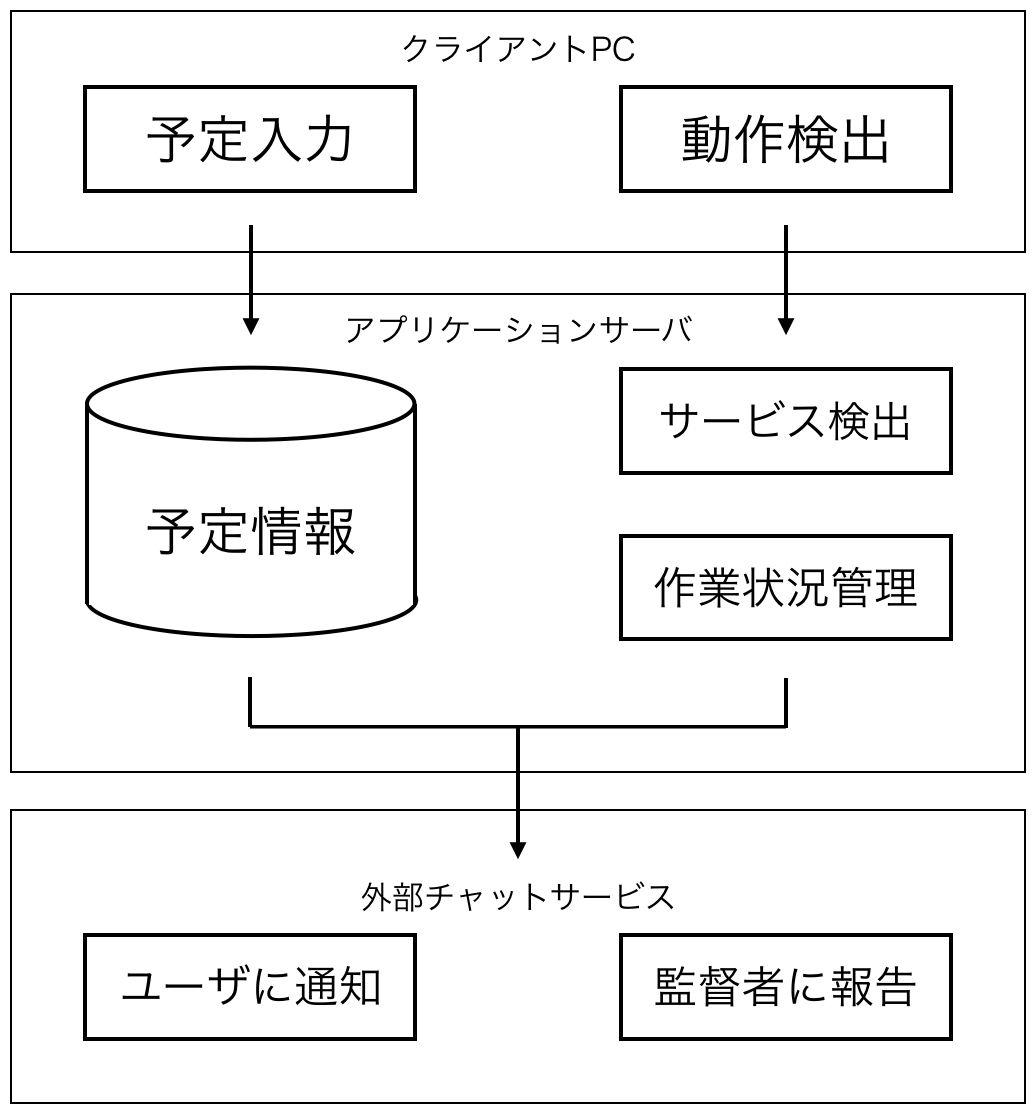
\includegraphics[width=8.0cm]{../graphics/structure_chart.png}
  \caption{システム構成図}
  \label{fig:structure_chart}
  \end{center}
\end{figure}

\section{実験}

この実験の目的は,ユーザと管理者両方の視点から有用性を測ることである.
まず,ユーザがシステムを利用することによって,作業の生産性が向上するかどうかを検証する.
また,管理者は,自動的に報告されるユーザの作業状況を確認し,現状を把握できるかどうかを確認する.

監視対象であるユーザは,論文を執筆する際にアプリケーションを起動する.
本システムは,起動中のアプリケーションから収集される情報をもとに,作業記録の生成を行う.
生成された作業記録は,次の日の朝に,チャットサービスを通じて管理者に送信される.
それらの一連の流れを確認することで,システム自体の信頼性や情報の適正性を測る.

システムの運用を行なった結果,ユーザが作成した予定を元に作業時間を記録し,自動的に報告を行うことができた.
ユーザが自身の作業を行うように促す効果があることも判明し,本システムの有用性が高いことが検証された.

\section{まとめと今後の課題}
本研究では,個人のPCワークの進捗管理により,生産性を向上させることを目標としたシステムを構築した.
実験では実際にシステムの運用を行い,利用者からの評価を受け,提案したシステムの有用性を測った.

システムの運用を行なった結果,ユーザが作成した予定を元に作業時間を記録し,自動的に報告を行うことができた.
これにより,ユーザが自身の作業を行うように促す効果があることが判明した.
また,報告される情報も,監督者も作業者の現状を確認し,指導に役立つものであると評価された.
以上のことより,本システムの有用性が高いことが検証された.

進捗監視システムをより現実的なものにするためには,より正確な予定の管理機能を実現することが重要である.
そのためには,信頼性が高く,ユーザにとってより使いやすいシステムにしていく必要がある.
また,組織で運用していく中で,システムを通じてコミュニケーションがとれるサービスとして進化させていくことにより,組織全体の生産性を向上させるものになると考える.

%%%%%%%%ここまで本文%%%%%%%%%%%%%%%%%%%%%%

\bibliographystyle{junsrt}
\bibliography{components/refs.bib}
%
\end{document}
